\setcounter{step}{0}
%------------------------------------------
% information doc
\subsection{Mäso s bylinkovým maslom}
\PrepTime{45}
\CookingTime{10}
\CookingTempe{180}
\TypeCooking{Praženie}
\NbPerson{4}
\Image{0 0 430 430}{images/florentin} %style 2
%------------------------------------------

\begin{ingredient}
%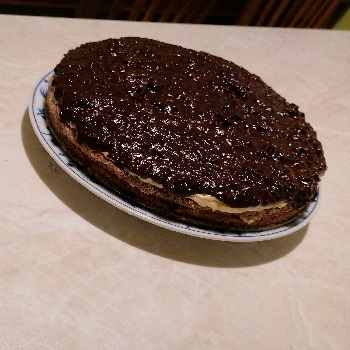
\includegraphics[height=5.5cm]{images/daim}
\def\portions{4}%
\textbf{{\normalsize Ingrediencie (\portions porcie):}}
%\vspace{0.5cm}
\begin{main}
	\item kuracie mäso
	\item PL maslo
	\item šunka
	\item cesnak
	\item pažitka
	\item trojobal
\end{main}
\end{ingredient}
\begin{recipe}
\textbf{{\normalsize Príprava:}}
\begin{enumerate}

\item{Maslo zmiešať s cesnakom a bylinkami urobiť guľku, a dať do mrazničky}
\item{Spraviť otvor do mäsa, kde vložíme v šunke zabalené maslo}
\item{Obaliť v trojobale}	
\item{Vypražiť}

\end{enumerate}
\end{recipe}

\begin{notes}

\end{notes}
\clearpage	